\chapter{The methylome as an encoding surface}\label{ch:surface}

\section{What $\beta$ measures}

At a single CpG on a single DNA molecule, methylation is binary: the cytosine carries a methyl group
or it does not. An array or a sequencing experiment never sees one molecule. It sees the DNA of
thousands to millions of cells, two alleles each, and reports the fraction $\beta$ of copies that
are methylated. So $\beta$ is a probability: the probability that a copy of that locus, drawn at
random from the specimen, is methylated.

That makes the entropy of a locus well defined. The Shannon entropy of a binary variable with
probability $\beta$ is
\begin{equation}
  H(\beta)=-\beta\log_2\beta-(1-\beta)\log_2(1-\beta),
  \label{eq:H}
\end{equation}
in bits. $H=0$ when every copy agrees (fully methylated or fully unmethylated) and $H=1$ bit when
the copies are split evenly, $\beta=\tfrac12$. \derived{} A locus is therefore an encoding site
whose capacity is one bit, and $H(\beta)$ says how much of that capacity the cells of the specimen are
using at that locus: how uncertain the pattern is, copy to copy.

\begin{remark}
$H(\beta)$ is an entropy over the \emph{copies in the specimen}. A single cell has two copies of an
autosomal locus, so its own $\beta$ takes only the values $0$, $\tfrac12$ and $1$. A $\beta$ of 0.73
in a sorted-cell specimen is a statement about many cells of that kind: 73~\% of their copies at
that locus are methylated. The readings of Chapters~\ref{ch:meta} and~\ref{ch:iama} are readings of this entropy over copies, and of its single-molecule counterpart.
\end{remark}

\section{Two channels}

$H$ is symmetric about $\tfrac12$, so the same entropy is reached at a $\beta$ below one half and at one above it
(Figure~\ref{fig:binent}). A cell holds two kinds of site: sites it keeps methylated, near $\beta=1$, and sites it keeps
unmethylated, near $\beta=0$. These are its two \emph{channels}. On the methylated channel, losing methylation (moving $\beta$
down toward $\tfrac12$) raises $H$; on the unmethylated channel, gaining methylation raises $H$. Both are moves toward maximum
uncertainty. The widespread loss of methylation across gene bodies and repeats and the gain at CpG islands seen together in
many tumours~\cite{Baylin2011} are, in this language, the same move on the two channels: the pattern becomes less certain.
\analogy{} for the tumour statement; the entropy statement itself is \derived.

\begin{figure}[htbp]\centering
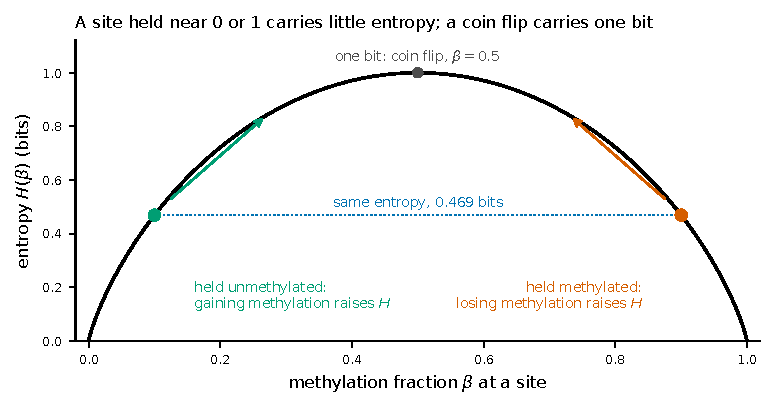
\includegraphics[width=0.95\textwidth]{figures/part4/fig_binary_entropy.pdf}
\caption{Binary entropy $H(\beta)$. A site held near $\beta=0$ or $\beta=1$ carries little entropy; a site at a coin flip
carries one bit. \calc}
\label{fig:binent}
\end{figure}

\section{The mean of the entropies}

A cell is read on a set of sites, not one. Two ways of combining them give different numbers. $H$ is concave, so by
Jensen's inequality
\begin{equation}
  H(\bbar)\ \ge\ \overline{H(\beta)},\qquad \bbar=\frac1n\sum_i\beta_i ,
  \label{eq:jensen}
\end{equation}
with equality only when all $\beta_i$ are equal. \derived{} On a set that holds both channels, the entropy of the mean is
meaningless: averaging a site at 0.9 with one at 0.1 gives $\bbar=\tfrac12$ and one bit, whatever the cell is doing. The
mean of the per-site entropies,
\begin{equation}
  \overline{H}=\frac1n\sum_i H(\beta_i),
  \label{eq:meanH}
\end{equation}
treats the two channels alike, because $H(\beta)=H(1-\beta)$, and it measures what the cell is doing at each site: how far
each site is from being held. This is the statistic of Met-A (Chapter~\ref{ch:meta}). It is read on \emph{identity sites},
chosen so that the cell's own healthy specimens hold them steadily, half on each channel (Chapter~\ref{ch:identity}).

On the 6,000 neutrophil identity sites the two ways of combining differ by a factor of three (Figure~\ref{fig:p4_jensen},
Table~\ref{tab:p4_jensen}). The mean of the per-site entropies is 0.330 bits, the healthy reference of Chapter~\ref{ch:meta}. The entropy of
the mean $\beta$ over both channels is 1.000 bit, whatever the cell is doing. Within one channel the two nearly agree (0.323 and
0.325 bits on the methylated channel), because the sites of one channel sit close together in $\beta$. \calc

\begin{figure}[htbp]\centering
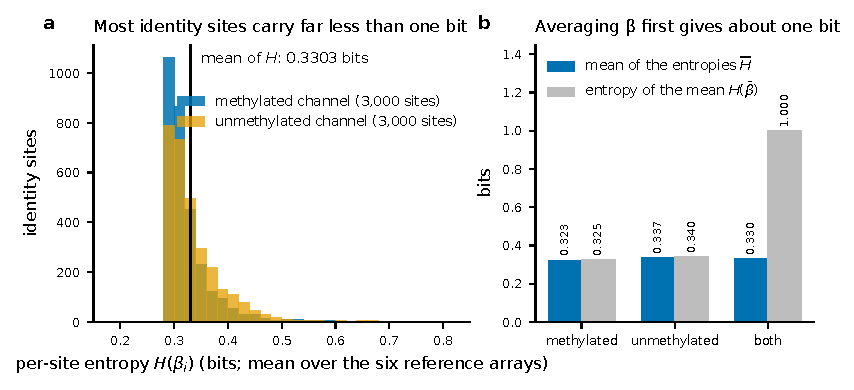
\includegraphics[width=0.95\textwidth]{figures/part4/fig_p4_03_jensen.pdf}
\caption{Jensen's inequality on the neutrophil identity sites. (a) Per-site entropy $H(\beta_i)$, averaged over the six reference arrays, for the
3,000 sites of each channel; the vertical line is their mean. (b) Mean of the entropies against the entropy of the mean $\beta$, per channel
and over both (channel assigned by the healthy mean $\beta$). \calc{} from the \calibrated{} reference.}
\label{fig:p4_jensen}
\end{figure}
\begin{table}[htbp]\centering\small
\caption{The mean of the entropies and the entropy of the mean on the 6,000 neutrophil identity sites (bits). \calc}\label{tab:p4_jensen}
\begin{tabular}{@{}lrrrr@{}}\toprule
sites & $n$ & mean $\beta$ & $H(\bar\beta)$ & $\overline{H}$ \\\midrule
methylated channel & 3,000 & 0.941 & 0.325 & 0.323 \\
unmethylated channel & 3,000 & 0.063 & 0.340 & 0.337 \\
both channels & 6,000 & 0.502 & 1.000 & 0.330 \\
\bottomrule
\end{tabular}
\end{table}

Averaging $H$ site by site has one cost: zero-mean array noise adds a positive bias at every site through the curvature of
$H$. The instrument meets it twice. The healthy reference is measured on the same platform through the same calibration, so
the bias of a typical array is in the denominator as well as the numerator. And the array's own noise is measured on every
specimen at the sites that every blood cell holds fixed (the noise index, Chapter~\ref{ch:instrument}).

\section{A capacity, and a ceiling}

A site's entropy cannot exceed one bit. A cell whose identity sites all sit at a coin flip has used the whole capacity of
that part of its surface. On the gauge of Chapter~\ref{ch:gauge} this is the far right end, the most error the gauge can show, and it has an exact
value for each cell type: one bit over the healthy reference. There is a second, earlier limit that matters for an
instrument. On the methylated channel $H$ rises as $\beta$ falls only while $\beta>\tfrac12$; past that, further loss lowers
$H$ again. A cell that has lost methylation past the half-way point therefore reads \emph{lower} on Met-A than one that has
lost less. The chain flags this and tells the reader to read the mean $\beta$ instead
(Chapter~\ref{ch:chain}). The DNA-methyltransferase-inhibitor series of Chapter~\ref{ch:firstreadings} shows it on real
arrays. \measured

\section{A pattern is a steady state}

A methylation pattern is not written once. At each division the maintenance machinery copies it
with finite fidelity, and between divisions de novo methyltransferases and TET-mediated oxidation
add and remove marks. The simplest model of a locus is a two-state chain per division: a methylated
copy stays methylated with probability $1-u$; an unmethylated copy becomes methylated with probability
$d$. Its steady state is
\begin{equation}
  \beta_{\mathrm{ss}}=\frac{d}{u+d}.
  \label{eq:steady}
\end{equation}
\derived{} With $u=0.03$ and $d=0.08$, $\beta_{\mathrm{ss}}=0.727$ and $H=0.845$ bits. \calc{} The model is too simple to
fit data, but it says what a held pattern is in mechanistic terms: the entropy a site settles at when writing and erasing
balance. A cell whose balance shifts, toward less faithful maintenance or more active removal, drifts toward $\beta=\tfrac12$
and its entropy rises. A cell whose copies agree with one another more than the healthy cell's do holds less entropy and
moves the other way. The gauge of Chapter~\ref{ch:gauge} reads both directions; what each direction
means for the cell is the subject of Chapter~\ref{ch:leukocyte}.

\section{Capacity of the surface}

With one bit of capacity per CpG copy, the methylation surface of one haploid human genome has a capacity of about
$2.8\times10^7$ bits. \calc{} The entropy actually carried is much less, because most CpGs are held near 0 or 1 and contribute
almost no entropy. The information the pattern holds is in which sites are held where. The \emph{entropy} the instrument
measures is something else: how uncertain the pattern is, on the sites that define a given cell.
